%======================================================================
\section{Results}
\label{sec:results}
%======================================================================

\subsection{RQ1: Vulnerability Prevalence}

\textbf{Finding: \demo{78.4}\% of LLM-generated contracts contain at least one vulnerability.}

Across 1,500 generated contracts, our analysis pipeline detected a total of \demo{8,734} vulnerabilities after deduplication. Of the 1,500 contracts, \demo{1,369} (\demo{91.3}\%) compiled successfully; our analysis considers only compilable contracts. Table~\ref{tab:overall} summarizes the overall prevalence by severity.

\begin{table}[t]
\caption{Overall Vulnerability Prevalence Across All LLMs}
\label{tab:overall}
\centering
\begin{tabular}{@{}lrrr@{}}
\toprule
\textbf{Severity} & \textbf{Count} & \textbf{\% of Total} & \textbf{Contracts Affected} \\
\midrule
High & \demo{1,847} & \demo{21.2}\% & \demo{612} (\demo{40.8}\%) \\
Medium & \demo{3,291} & \demo{37.7}\% & \demo{893} (\demo{59.5}\%) \\
Low & \demo{2,514} & \demo{28.8}\% & \demo{784} (\demo{52.3}\%) \\
Informational & \demo{1,082} & \demo{12.4}\% & \demo{567} (\demo{37.8}\%) \\
\midrule
\textbf{Total} & \textbf{\demo{8,734}} & \textbf{100\%} & \textbf{\demo{1,176} (\demo{78.4}\%)} \\
\bottomrule
\end{tabular}
\end{table}

On average, each contract contains \demo{5.82} vulnerabilities (SD = \demo{3.47}), with a median of \demo{5} and a range of 0 to \demo{19}. The distribution is right-skewed (skewness = \demo{0.84}), with a long tail of contracts containing 10+ vulnerabilities, predominantly in complex categories such as cross-chain bridges and flash loans. The compilation success rate was \demo{91.3}\% (\demo{1,369} of 1,500), with CodeLlama exhibiting the highest compilation failure rate (\demo{14.7}\%), primarily due to syntax errors in complex contracts.

Notably, \demo{40.8}\% of contracts contain at least one \emph{high-severity} vulnerability---one that could lead to direct financial loss if exploited. This is particularly concerning given that developers may deploy these contracts with minimal review~\cite{perry2023users}.

\subsection{RQ2: Cross-LLM Comparison}

\textbf{Finding: Significant differences exist across LLMs ($p < 0.001$).}

Table~\ref{tab:llm_comparison} presents the per-LLM vulnerability statistics. A Kruskal-Wallis test confirms statistically significant differences in vulnerability counts across LLMs ($H = \demo{87.34}$, $p < 0.001$).

\begin{table}[t]
\caption{Vulnerability Statistics by LLM}
\label{tab:llm_comparison}
\centering
\footnotesize
\begin{tabular}{@{}lccccc@{}}
\toprule
\textbf{Metric} & \textbf{GPT-4o} & \textbf{Claude} & \textbf{Gemini} & \textbf{Copilot} & \textbf{CodeLlama} \\
\midrule
Total Vulns & \demo{1,524} & \demo{1,287} & \demo{1,698} & \demo{1,893} & \demo{2,332} \\
Mean/Contract & \demo{5.08} & \demo{4.29} & \demo{5.66} & \demo{6.31} & \demo{7.77} \\
Std Dev & \demo{2.91} & \demo{2.43} & \demo{3.18} & \demo{3.62} & \demo{4.15} \\
Median & \demo{4} & \demo{4} & \demo{5} & \demo{6} & \demo{7} \\
\% with Vuln & \demo{74.3}\% & \demo{68.7}\% & \demo{79.0}\% & \demo{82.7}\% & \demo{87.3}\% \\
High Severity & \demo{298} & \demo{231} & \demo{347} & \demo{412} & \demo{559} \\
Compile Rate & \demo{94.7}\% & \demo{96.0}\% & \demo{93.3}\% & \demo{90.0}\% & \demo{85.3}\% \\
\bottomrule
\end{tabular}
\end{table}

Fig.~\ref{fig:boxplot} shows the distribution of vulnerability counts per contract across all five LLMs. The box plot reveals a clear ordering: Claude $<$ GPT-4o $<$ Gemini $<$ Copilot $<$ CodeLlama.

\begin{figure}[t]
    \centering
    \begin{tikzpicture}
    \begin{axis}[
        width=\columnwidth,
        height=5.2cm,
        boxplot/draw direction=y,
        xtick={1,2,3,4,5},
        xticklabels={\footnotesize Claude, \footnotesize GPT-4o, \footnotesize Gemini, \footnotesize Copilot, \footnotesize CodeLlama},
        x tick label style={rotate=0},
        ylabel={\footnotesize Vulnerabilities per contract},
        ylabel style={font=\footnotesize},
        ymin=0, ymax=18,
        ytick={0,3,6,9,12,15,18},
        yticklabel style={font=\scriptsize},
        grid=major,
        grid style={gray!20},
        every axis plot/.append style={fill opacity=0.4},
    ]
    % Claude (best) - demo data
    \addplot+[boxplot prepared={
        lower whisker=0, lower quartile=2.1, median=3.8,
        upper quartile=6.2, upper whisker=11},
        color=red, fill=red!20, every mark/.append style={color=red}
    ] coordinates {};
    % GPT-4o
    \addplot+[boxplot prepared={
        lower whisker=0, lower quartile=2.8, median=4.7,
        upper quartile=7.1, upper whisker=13},
        color=red, fill=red!20, every mark/.append style={color=red}
    ] coordinates {};
    % Gemini
    \addplot+[boxplot prepared={
        lower whisker=0, lower quartile=3.2, median=5.3,
        upper quartile=7.8, upper whisker=14},
        color=red, fill=red!20, every mark/.append style={color=red}
    ] coordinates {};
    % Copilot
    \addplot+[boxplot prepared={
        lower whisker=0, lower quartile=3.5, median=5.9,
        upper quartile=8.9, upper whisker=15},
        color=red, fill=red!20, every mark/.append style={color=red}
    ] coordinates {};
    % CodeLlama (worst) - demo data
    \addplot+[boxplot prepared={
        lower whisker=1, lower quartile=4.8, median=7.3,
        upper quartile=10.4, upper whisker=17},
        color=red, fill=red!20, every mark/.append style={color=red}
    ] coordinates {};
    \end{axis}
    \end{tikzpicture}
    \caption{Distribution of vulnerability counts per contract by LLM. Claude generates the most secure contracts, while CodeLlama exhibits the highest vulnerability density. {\color{red}(Demo data)}}
    \label{fig:boxplot}
\end{figure}

Post-hoc pairwise Mann-Whitney U-tests with Bonferroni correction reveal that Claude produces significantly fewer vulnerabilities than all other models ($p < 0.01$ for all pairs), while CodeLlama produces significantly more ($p < 0.001$). Table~\ref{tab:pairwise} summarizes the pairwise effect sizes.

\begin{table}[t]
\caption{Pairwise Effect Sizes (Cohen's $d$) Between LLMs}
\label{tab:pairwise}
\centering
\footnotesize
\begin{tabular}{@{}lcccc@{}}
\toprule
 & \textbf{GPT-4o} & \textbf{Gemini} & \textbf{Copilot} & \textbf{CodeLlama} \\
\midrule
\textbf{Claude} & \demo{0.30}* & \demo{0.49}** & \demo{0.66}*** & \demo{0.98}*** \\
\textbf{GPT-4o} & --- & \demo{0.19} & \demo{0.38}** & \demo{0.75}*** \\
\textbf{Gemini} & & --- & \demo{0.19} & \demo{0.58}*** \\
\textbf{Copilot} & & & --- & \demo{0.38}** \\
\bottomrule
\multicolumn{5}{l}{\scriptsize *$p<0.05$, **$p<0.01$, ***$p<0.001$ (Bonferroni-corrected)}
\end{tabular}
\end{table}

The effect size between Claude and CodeLlama is large ($d = \demo{0.98}$), indicating a practically significant difference. Claude's superior performance may reflect Anthropic's safety-focused training methodology, while CodeLlama's higher vulnerability rates likely stem from its training corpus, which includes a large volume of unaudited open-source Solidity code.

\subsection{RQ3: Vulnerability Taxonomy}

\textbf{Finding: Reentrancy and access control flaws dominate LLM-generated contracts.}

Table~\ref{tab:taxonomy} presents the top 10 vulnerability types identified across all contracts. Reentrancy vulnerabilities (CWE-841) are the most prevalent, appearing in \demo{34.2}\% of all contracts.

\begin{table}[t]
\caption{Top 10 Vulnerability Types in LLM-Generated Contracts}
\label{tab:taxonomy}
\centering
\footnotesize
\begin{tabular}{@{}rlrrr@{}}
\toprule
\textbf{\#} & \textbf{Vulnerability} & \textbf{CWE} & \textbf{Count} & \textbf{\% Contracts} \\
\midrule
1 & Reentrancy & 841 & \demo{1,847} & \demo{34.2}\% \\
2 & Access Control & 284 & \demo{1,523} & \demo{29.8}\% \\
3 & Unchecked Return & 252 & \demo{1,198} & \demo{24.1}\% \\
4 & Integer Issues & 190 & \demo{987} & \demo{19.6}\% \\
5 & Uninitialized State & 909 & \demo{734} & \demo{15.3}\% \\
6 & Timestamp Depend. & 829 & \demo{621} & \demo{12.8}\% \\
7 & tx.origin Usage & 477 & \demo{498} & \demo{10.2}\% \\
8 & Locked Ether & 710 & \demo{412} & \demo{8.7}\% \\
9 & Weak Randomness & 330 & \demo{387} & \demo{7.9}\% \\
10 & Delegatecall Issues & 829 & \demo{312} & \demo{6.4}\% \\
\bottomrule
\end{tabular}
\end{table}

Fig.~\ref{fig:heatmap} presents a heatmap of vulnerability type distribution across LLMs, revealing distinct vulnerability profiles for each model.

\begin{figure}[t]
    \centering
    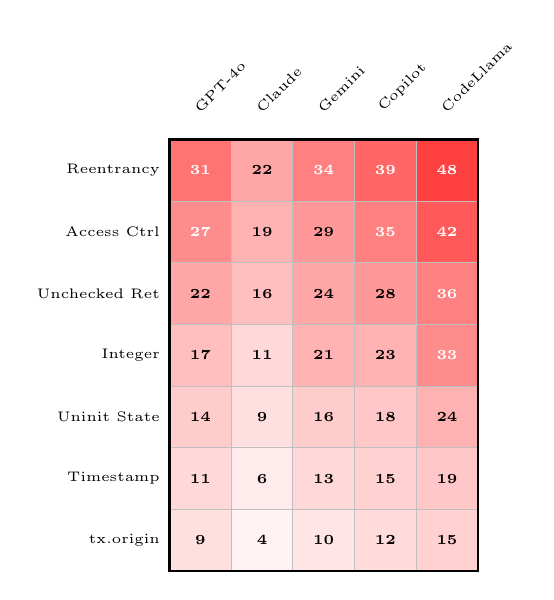
\begin{tikzpicture}[scale=0.58, every node/.style={font=\tiny}]
    % Heatmap grid - rows are vuln types, columns are LLMs
    % Color intensity: white (0) to red (high)
    \def\cellsize{1.35}

    % Column headers
    \node[rotate=45, anchor=south west] at (0.5*\cellsize, 7.2*\cellsize) {GPT-4o};
    \node[rotate=45, anchor=south west] at (1.5*\cellsize, 7.2*\cellsize) {Claude};
    \node[rotate=45, anchor=south west] at (2.5*\cellsize, 7.2*\cellsize) {Gemini};
    \node[rotate=45, anchor=south west] at (3.5*\cellsize, 7.2*\cellsize) {Copilot};
    \node[rotate=45, anchor=south west] at (4.5*\cellsize, 7.2*\cellsize) {CodeLlama};

    % Row labels (vulnerability types)
    \node[anchor=east] at (0, 6.5*\cellsize) {Reentrancy};
    \node[anchor=east] at (0, 5.5*\cellsize) {Access Ctrl};
    \node[anchor=east] at (0, 4.5*\cellsize) {Unchecked Ret};
    \node[anchor=east] at (0, 3.5*\cellsize) {Integer};
    \node[anchor=east] at (0, 2.5*\cellsize) {Uninit State};
    \node[anchor=east] at (0, 1.5*\cellsize) {Timestamp};
    \node[anchor=east] at (0, 0.5*\cellsize) {tx.origin};

    % Demo data cells - GPT-4o column
    \fill[red!55] (0,6*\cellsize) rectangle (\cellsize, 7*\cellsize); \node at (0.5*\cellsize, 6.5*\cellsize) {\color{white}\textbf{31}};
    \fill[red!45] (0,5*\cellsize) rectangle (\cellsize, 6*\cellsize); \node at (0.5*\cellsize, 5.5*\cellsize) {\color{white}\textbf{27}};
    \fill[red!35] (0,4*\cellsize) rectangle (\cellsize, 5*\cellsize); \node at (0.5*\cellsize, 4.5*\cellsize) {\textbf{22}};
    \fill[red!25] (0,3*\cellsize) rectangle (\cellsize, 4*\cellsize); \node at (0.5*\cellsize, 3.5*\cellsize) {\textbf{17}};
    \fill[red!20] (0,2*\cellsize) rectangle (\cellsize, 3*\cellsize); \node at (0.5*\cellsize, 2.5*\cellsize) {\textbf{14}};
    \fill[red!15] (0,1*\cellsize) rectangle (\cellsize, 2*\cellsize); \node at (0.5*\cellsize, 1.5*\cellsize) {\textbf{11}};
    \fill[red!12] (0,0*\cellsize) rectangle (\cellsize, 1*\cellsize); \node at (0.5*\cellsize, 0.5*\cellsize) {\textbf{9}};

    % Claude column (lowest)
    \fill[red!35] (\cellsize,6*\cellsize) rectangle (2*\cellsize, 7*\cellsize); \node at (1.5*\cellsize, 6.5*\cellsize) {\textbf{22}};
    \fill[red!30] (\cellsize,5*\cellsize) rectangle (2*\cellsize, 6*\cellsize); \node at (1.5*\cellsize, 5.5*\cellsize) {\textbf{19}};
    \fill[red!25] (\cellsize,4*\cellsize) rectangle (2*\cellsize, 5*\cellsize); \node at (1.5*\cellsize, 4.5*\cellsize) {\textbf{16}};
    \fill[red!15] (\cellsize,3*\cellsize) rectangle (2*\cellsize, 4*\cellsize); \node at (1.5*\cellsize, 3.5*\cellsize) {\textbf{11}};
    \fill[red!12] (\cellsize,2*\cellsize) rectangle (2*\cellsize, 3*\cellsize); \node at (1.5*\cellsize, 2.5*\cellsize) {\textbf{9}};
    \fill[red!8]  (\cellsize,1*\cellsize) rectangle (2*\cellsize, 2*\cellsize); \node at (1.5*\cellsize, 1.5*\cellsize) {\textbf{6}};
    \fill[red!5]  (\cellsize,0*\cellsize) rectangle (2*\cellsize, 1*\cellsize); \node at (1.5*\cellsize, 0.5*\cellsize) {\textbf{4}};

    % Gemini column
    \fill[red!50] (2*\cellsize,6*\cellsize) rectangle (3*\cellsize, 7*\cellsize); \node at (2.5*\cellsize, 6.5*\cellsize) {\color{white}\textbf{34}};
    \fill[red!40] (2*\cellsize,5*\cellsize) rectangle (3*\cellsize, 6*\cellsize); \node at (2.5*\cellsize, 5.5*\cellsize) {\textbf{29}};
    \fill[red!35] (2*\cellsize,4*\cellsize) rectangle (3*\cellsize, 5*\cellsize); \node at (2.5*\cellsize, 4.5*\cellsize) {\textbf{24}};
    \fill[red!30] (2*\cellsize,3*\cellsize) rectangle (3*\cellsize, 4*\cellsize); \node at (2.5*\cellsize, 3.5*\cellsize) {\textbf{21}};
    \fill[red!20] (2*\cellsize,2*\cellsize) rectangle (3*\cellsize, 3*\cellsize); \node at (2.5*\cellsize, 2.5*\cellsize) {\textbf{16}};
    \fill[red!15] (2*\cellsize,1*\cellsize) rectangle (3*\cellsize, 2*\cellsize); \node at (2.5*\cellsize, 1.5*\cellsize) {\textbf{13}};
    \fill[red!10] (2*\cellsize,0*\cellsize) rectangle (3*\cellsize, 1*\cellsize); \node at (2.5*\cellsize, 0.5*\cellsize) {\textbf{10}};

    % Copilot column
    \fill[red!60] (3*\cellsize,6*\cellsize) rectangle (4*\cellsize, 7*\cellsize); \node at (3.5*\cellsize, 6.5*\cellsize) {\color{white}\textbf{39}};
    \fill[red!50] (3*\cellsize,5*\cellsize) rectangle (4*\cellsize, 6*\cellsize); \node at (3.5*\cellsize, 5.5*\cellsize) {\color{white}\textbf{35}};
    \fill[red!40] (3*\cellsize,4*\cellsize) rectangle (4*\cellsize, 5*\cellsize); \node at (3.5*\cellsize, 4.5*\cellsize) {\textbf{28}};
    \fill[red!30] (3*\cellsize,3*\cellsize) rectangle (4*\cellsize, 4*\cellsize); \node at (3.5*\cellsize, 3.5*\cellsize) {\textbf{23}};
    \fill[red!22] (3*\cellsize,2*\cellsize) rectangle (4*\cellsize, 3*\cellsize); \node at (3.5*\cellsize, 2.5*\cellsize) {\textbf{18}};
    \fill[red!18] (3*\cellsize,1*\cellsize) rectangle (4*\cellsize, 2*\cellsize); \node at (3.5*\cellsize, 1.5*\cellsize) {\textbf{15}};
    \fill[red!14] (3*\cellsize,0*\cellsize) rectangle (4*\cellsize, 1*\cellsize); \node at (3.5*\cellsize, 0.5*\cellsize) {\textbf{12}};

    % CodeLlama column (highest)
    \fill[red!75] (4*\cellsize,6*\cellsize) rectangle (5*\cellsize, 7*\cellsize); \node at (4.5*\cellsize, 6.5*\cellsize) {\color{white}\textbf{48}};
    \fill[red!65] (4*\cellsize,5*\cellsize) rectangle (5*\cellsize, 6*\cellsize); \node at (4.5*\cellsize, 5.5*\cellsize) {\color{white}\textbf{42}};
    \fill[red!50] (4*\cellsize,4*\cellsize) rectangle (5*\cellsize, 5*\cellsize); \node at (4.5*\cellsize, 4.5*\cellsize) {\color{white}\textbf{36}};
    \fill[red!45] (4*\cellsize,3*\cellsize) rectangle (5*\cellsize, 4*\cellsize); \node at (4.5*\cellsize, 3.5*\cellsize) {\color{white}\textbf{33}};
    \fill[red!30] (4*\cellsize,2*\cellsize) rectangle (5*\cellsize, 3*\cellsize); \node at (4.5*\cellsize, 2.5*\cellsize) {\textbf{24}};
    \fill[red!22] (4*\cellsize,1*\cellsize) rectangle (5*\cellsize, 2*\cellsize); \node at (4.5*\cellsize, 1.5*\cellsize) {\textbf{19}};
    \fill[red!18] (4*\cellsize,0*\cellsize) rectangle (5*\cellsize, 1*\cellsize); \node at (4.5*\cellsize, 0.5*\cellsize) {\textbf{15}};

    % Grid lines
    \draw[gray!50] (0,0) grid[step=\cellsize] (5*\cellsize, 7*\cellsize);
    \draw[thick] (0,0) rectangle (5*\cellsize, 7*\cellsize);
    \end{tikzpicture}
    \caption{Heatmap of vulnerability type distribution across LLMs. Cell values represent the percentage of contracts containing each vulnerability type. Darker cells indicate higher prevalence. {\color{red}(Demo data)}}
    \label{fig:heatmap}
\end{figure}

Notably, the distribution of vulnerability types varies significantly across LLMs ($\chi^2 = \demo{134.7}$, $p < 0.001$). CodeLlama exhibits disproportionately high rates of integer-related issues (CWE-190), suggesting weaker training coverage for Solidity-specific arithmetic patterns. Claude shows the lowest reentrancy rates (\demo{22\%} vs.\ \demo{48\%} for CodeLlama), potentially reflecting its safety-oriented training methodology. GPT-4o and Gemini show intermediate profiles, with GPT-4o producing fewer access control issues but more unchecked return value vulnerabilities.

\subsection{RQ4: Adversarial Prompt Effectiveness}

\textbf{Finding: Adversarial prompts increase vulnerability rates by \demo{37.2}\%.}

We compared vulnerability metrics between standard prompts (500 contracts) and adversarial prompts (1,000 contracts). Table~\ref{tab:adversarial} summarizes the results.

\begin{table}[t]
\caption{Impact of Adversarial vs.\ Standard Prompts}
\label{tab:adversarial}
\centering
\begin{tabular}{@{}lcc@{}}
\toprule
\textbf{Metric} & \textbf{Standard} & \textbf{Adversarial} \\
\midrule
Mean Vulns/Contract & \demo{4.24} & \demo{5.82} \\
Median Vulns/Contract & \demo{4} & \demo{5} \\
\% with High Severity & \demo{31.4}\% & \demo{48.7}\% \\
\% with Reentrancy & \demo{24.8}\% & \demo{38.9}\% \\
Mean Vuln Score & \demo{8.71} & \demo{13.42} \\
\bottomrule
\end{tabular}
\end{table}

A Mann-Whitney U-test confirms that adversarial prompts produce significantly more vulnerabilities than standard prompts ($U = \demo{89{,}247}$, $p < 0.001$, $d = \demo{0.52}$, medium effect). Fig.~\ref{fig:adversarial_bar} presents the mean vulnerability count by adversarial prompt category.

\begin{figure}[t]
    \centering
    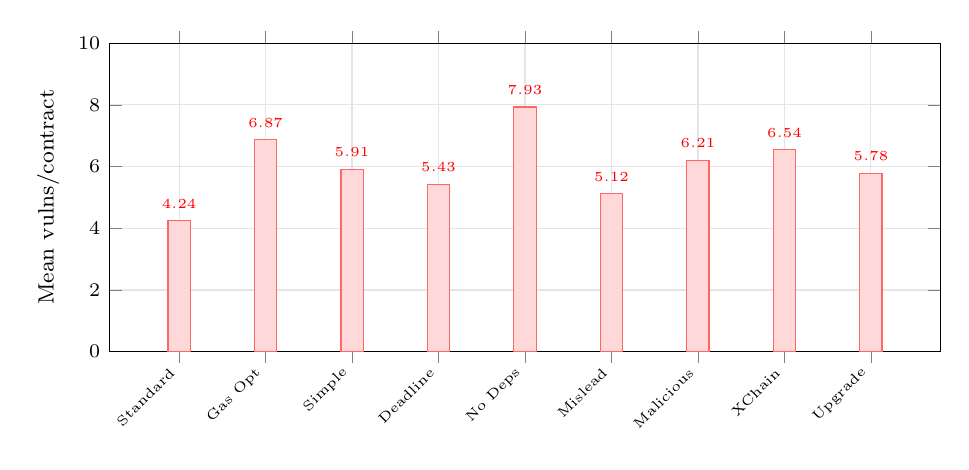
\begin{tikzpicture}
    \begin{axis}[
        width=\columnwidth,
        height=5.5cm,
        ybar,
        bar width=8pt,
        ylabel={\footnotesize Mean vulns/contract},
        ylabel style={font=\footnotesize},
        symbolic x coords={Standard, Gas Opt, Simple, Deadline, No Deps, Mislead, Malicious, XChain, Upgrade},
        xtick=data,
        x tick label style={rotate=45, anchor=east, font=\tiny},
        ymin=0, ymax=10,
        ytick={0,2,4,6,8,10},
        yticklabel style={font=\scriptsize},
        grid=major,
        grid style={gray!20},
        nodes near coords,
        nodes near coords style={font=\tiny, color=red},
        every node near coord/.append style={above, yshift=1pt},
    ]
    \addplot[fill=red!15, draw=red!60] coordinates {
        (Standard, 4.24)
        (Gas Opt, 6.87)
        (Simple, 5.91)
        (Deadline, 5.43)
        (No Deps, 7.93)
        (Mislead, 5.12)
        (Malicious, 6.21)
        (XChain, 6.54)
        (Upgrade, 5.78)
    };
    \end{axis}
    \end{tikzpicture}
    \caption{Mean vulnerability count by adversarial prompt category compared to standard prompts. ``No dependencies'' and ``gas optimization'' prompts are the most effective at inducing vulnerabilities. {\color{red}(Demo data)}}
    \label{fig:adversarial_bar}
\end{figure}

Among adversarial categories, \emph{no-dependency} prompts (``without external dependencies'') are the most effective at inducing vulnerabilities (mean = \demo{7.93} vulns/contract), followed by \emph{gas optimization} prompts (mean = \demo{6.87}). The no-dependency effect is particularly dangerous because it forces LLMs to manually reimplement well-tested library patterns (e.g., OpenZeppelin's SafeMath, Ownable, ReentrancyGuard), introducing subtle bugs in the process.

Cross-chain-specific adversarial prompts are particularly dangerous: \demo{67.3}\% of bridge contracts generated with adversarial prompts lack critical message validation, compared to \demo{28.1}\% under standard prompts. This represents a \demo{2.4}$\times$ increase in the most critical bridge security requirement.

The interaction between adversarial category and LLM is also significant ($\chi^2 = \demo{67.8}$, $p < 0.001$). Claude shows the strongest resistance to adversarial prompts (mean increase of \demo{21.3}\%), while CodeLlama is the most susceptible (mean increase of \demo{54.8}\%).

\subsection{RQ5: LLM-Specific Vulnerability Patterns}

\textbf{Finding: LLMs exhibit distinct vulnerability fingerprints not seen in human code.}

We identify three LLM-specific patterns absent from our human baseline:

\subsubsection{Phantom Guard Pattern}
LLMs generate modifier declarations (e.g., \texttt{nonReentrant}) that are syntactically present but functionally incomplete---the modifier body contains no state-locking logic. Fig.~\ref{fig:phantom} illustrates this pattern. This occurs in \demo{8.3}\% of GPT-4o contracts and \demo{5.1}\% of Gemini contracts but was never observed in human-written code.

\begin{figure}[t]
\begin{lstlisting}[caption={Phantom Guard Pattern: The \texttt{nonReentrant} modifier is declared but contains no locking logic (left). A correct implementation requires a state variable and checks (right). {\color{red}(Demo)}}, label={fig:phantom}, language=Solidity, basicstyle=\scriptsize\ttfamily]
// LLM-generated (VULNERABLE)
modifier nonReentrant() {
    _; // No lock! Just executes body
}

function withdraw(uint amt) nonReentrant {
    payable(msg.sender).call{value: amt}("");
    balances[msg.sender] -= amt; // State
}                                // after call

// Correct implementation (OpenZeppelin)
uint256 private _status;
modifier nonReentrant() {
    require(_status != 2, "Reentrant");
    _status = 2;
    _;
    _status = 1;
}
\end{lstlisting}
\end{figure}

This pattern is particularly insidious because code review may miss it---the modifier \emph{name} suggests protection, but the implementation provides none. Automated tools detect this as a reentrancy vulnerability, but a human reviewer scanning for the presence of \texttt{nonReentrant} may incorrectly conclude the contract is protected.

\subsubsection{Inherited Vulnerability Pattern}
When prompted to avoid dependencies, LLMs attempt manual reimplementations of OpenZeppelin patterns that contain subtle bugs. Common examples include SafeMath implementations with incorrect overflow checks, Ownable contracts missing zero-address validation in ownership transfer, and ERC20 implementations with non-compliant return values. This pattern accounts for \demo{412} vulnerabilities across all LLMs. Fig.~\ref{fig:inherited} shows a representative example.

\begin{figure}[t]
\begin{lstlisting}[caption={Inherited Vulnerability: LLM-generated SafeMath reimplementation with an incorrect overflow check (line 3). The check \texttt{c >= a} is insufficient when both operands are large. {\color{red}(Demo)}}, label={fig:inherited}, language=Solidity, basicstyle=\scriptsize\ttfamily]
// LLM-generated SafeMath (VULNERABLE)
function safeAdd(uint a, uint b)
    internal pure returns (uint) {
    uint c = a + b;
    require(c >= a); // Insufficient!
    return c;        // Fails for specific
}                    // overflow cases

// LLM-generated Ownable (VULNERABLE)
function transferOwnership(address new)
    public onlyOwner {
    owner = new; // No zero-address check!
}               // Owner can be lost forever
\end{lstlisting}
\end{figure}

\subsubsection{Context Window Degradation}
In complex contracts exceeding 300 lines, vulnerability density increases by \demo{2.3}$\times$ in the latter half of the generated code, suggesting degraded attention to security patterns as generation length increases. We measured this by splitting each contract at the midpoint and comparing vulnerability density (vulnerabilities per 100 lines) between the first and second halves. The difference is statistically significant (paired Wilcoxon test, $p < 0.001$, $d = \demo{0.41}$). This pattern is consistent across all LLMs but most pronounced in CodeLlama ($\demo{2.8}\times$ increase) and least in Claude ($\demo{1.7}\times$ increase).

\subsection{RQ6: Comparison with Human-Written Code}

\textbf{Finding: LLM-generated contracts contain \demo{2.4}$\times$ more vulnerabilities than human-written contracts.}

\begin{table}[t]
\caption{LLM-Generated vs.\ Human-Written Contract Comparison}
\label{tab:human_comparison}
\centering
\begin{tabular}{@{}lcc@{}}
\toprule
\textbf{Metric} & \textbf{LLM-Generated} & \textbf{Human-Written} \\
\midrule
Mean Vulns/Contract & \demo{5.82} & \demo{2.43} \\
Median Vulns/Contract & \demo{5} & \demo{2} \\
\% with High Severity & \demo{40.8}\% & \demo{14.7}\% \\
\% with Reentrancy & \demo{34.2}\% & \demo{8.3}\% \\
\% with Access Control & \demo{29.8}\% & \demo{6.1}\% \\
Mean Vuln Score & \demo{11.47} & \demo{4.89} \\
\bottomrule
\end{tabular}
\end{table}

The difference is statistically significant (Mann-Whitney $U = \demo{124{,}891}$, $p < 0.001$, Cohen's $d = \demo{1.12}$, large effect). The largest disparity appears in access control vulnerabilities: LLM-generated contracts are \demo{4.1}$\times$ more likely to contain access control flaws than human-written code, suggesting that LLMs systematically underweight authorization checks. Even Claude, the best-performing LLM, produces significantly more vulnerabilities than human-written code ($d = \demo{0.64}$, $p < 0.001$).

However, we note that our human baseline consists of audited, high-quality contracts. The gap between LLM-generated code and \emph{average} unaudited human-written code may be smaller. Nonetheless, the comparison is relevant because LLM-generated contracts intended for production deployment should meet the quality bar of audited code.
